\documentclass{scrartcl}
\usepackage[a4paper,left=1in,right=1in,top=1.2in,bottom=1in]{geometry}
\usepackage{siunitx}
\usepackage{graphicx}
\setkomafont{disposition}{\normalfont\bfseries}
\usepackage{amsmath}
\usepackage{easytable}
\usepackage{lipsum}
\usepackage{ragged2e}
\allowdisplaybreaks

%title
\title{Extra assignment:\\Inference for continuous detection and discrimination}
\subtitle{Theoretical Neuroscience II}
\author{Johannes G\"atjen}


\begin{document}
\maketitle

\section{Maximum joint density/probability}
\label{maxes}

I determined the peak density of the joint probability density function with three different computational methods.\footnote{I also tried to derive the maximum directly (analytically) from the probability density function, but gave up after still getting apparently wrong results after multiple attempts. One result included $c_s = -c_0$, another gave $x_k = \sqrt{\frac{1}{2\pi}}, \theta_s = \theta_k, c_s= \frac{c_0}{2} + \sqrt{\frac{c_0^2}{4}+\frac{c_0}{8e^2}}$} The results are summed up in the following table. For the first method, I wrote a function that evaluates the pdf directly and used a library function to iteratively find the maximum. For the second method I sampled the same function at fixed points at linearly spaced values for $\theta_k$ and logarithmically spaced values for $x_k$ and $c_s$, and selected the maximum from those results. Transforming the density function into a probability function, I also obtained an analytic result for the peak (discretized) probability. Lastly I generated stimuli and responses according to the probability distributions and calculated the empirical/numerical peak density and probability from the results. The chosen parameters are $c_0 = 1$ and $\theta_k = 0$. 


\centering
\begin{TAB}(r, 10pt, 20pt)[4pt]{cc|c|c|c}{c|ccc|cc}
& \textbf{Method} & $\mathbf{x_k}$ & $\mathbf{c_s}$ & $\mathbf{\theta_s}$ \\
\textbf{peak density}	& direct optimization	& $\approx\num{1e-100}$ & $\approx\num{1e-100}$ & $\approx 3.7$ \\
& analytic & \num{1e-8} & \num{2e-8} & 2 \\
& numeric & 0 & \num{3e-8}  & 3.7\\
\textbf{peak probability}& analytic & 10 & 1 & 0 \\	
& numeric & 7.3 & 0.65 & 0 \\	
\end{TAB}

\justify
The results for the location of the peak probability do not agree closely for the response and contrast, but are within an order of magnitude. Since they are on a logarithmic scale, we cannot expect much better.

The results for the peak density show $x_k$ and $c_s$ close to zero. However the density function with $x_k = 0$ is equal to zero (so not maximal), and it is not defined for $c_s = 0$. The response rate $x_k$ is Rayleigh distributed with a mean determined by the stimulus contrast $c_s$ and orientation $\theta_s$. The mean tends towards zero with $c_s$. A Rayleigh distribution with the mean tending towards zero degenerates into a Dirac delta function $\operatorname{\delta}(x - \epsilon)$. This means the density at that point tends to infinity.

\section{Marginal response distribution}

Figure \ref{margs} shows the marginal distribution of the response rate, once derived analytically, once numerically, as described in Section \ref{maxes}. Qualitatively the analytic and numeric solutions agree well. The absolute values for the numeric solution are a bit smaller than for the analytic solution.

\begin{figure}[h]
\centering
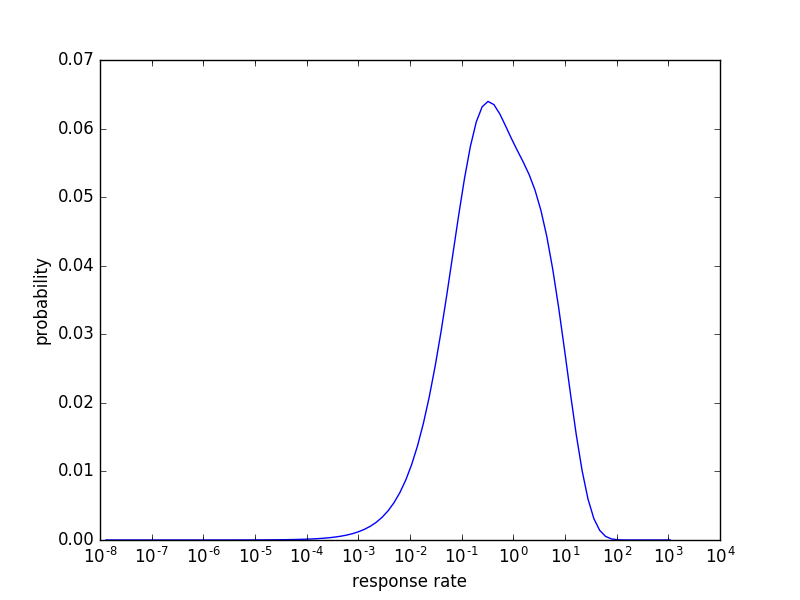
\includegraphics[width=0.47\textwidth, clip]{../pics/s2/margXProb_analytic_final}
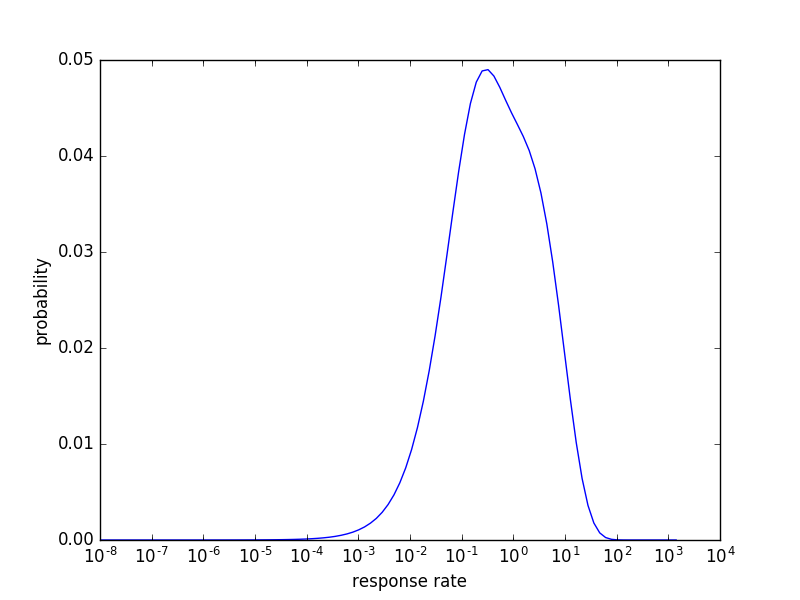
\includegraphics[width=0.47\textwidth, clip]{../pics/s2/margXProb_numeric_final} \\
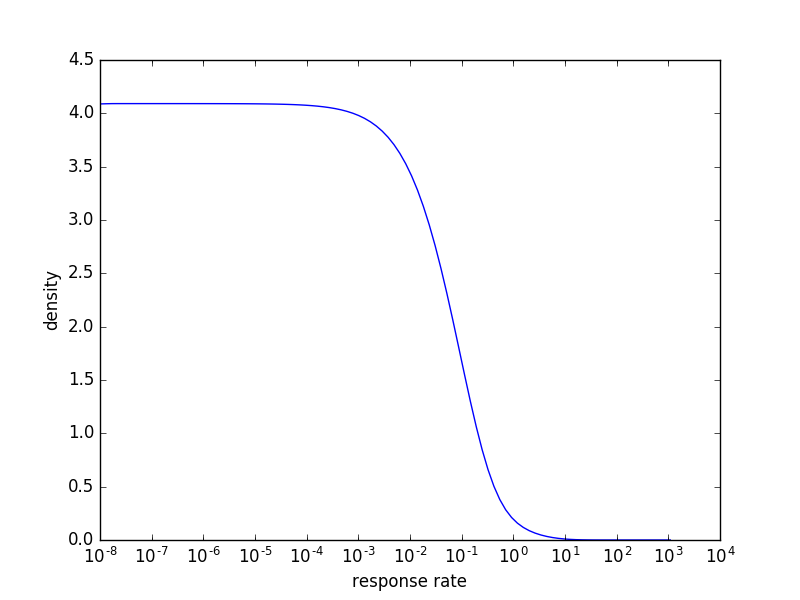
\includegraphics[width=0.47\textwidth, clip]{../pics/s2/margXDens_analytic_final}
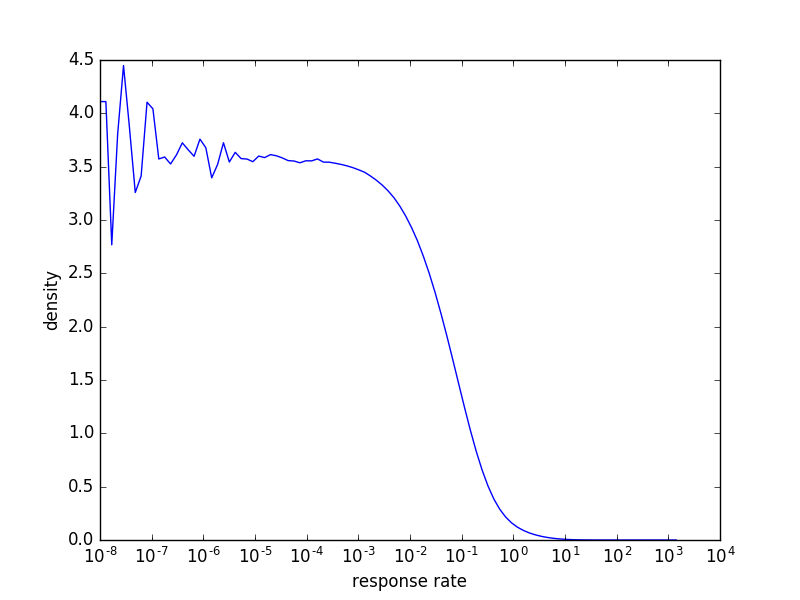
\includegraphics[width=0.47\textwidth, clip]{../pics/s2/margXDens_numeric_final}\\
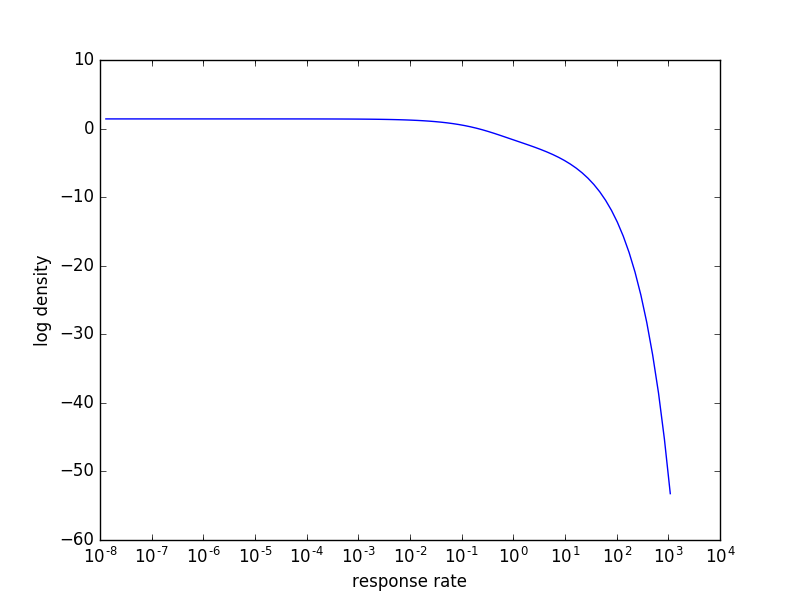
\includegraphics[width=0.47\textwidth, clip]{../pics/s2/margXLogDens_analytic_final}
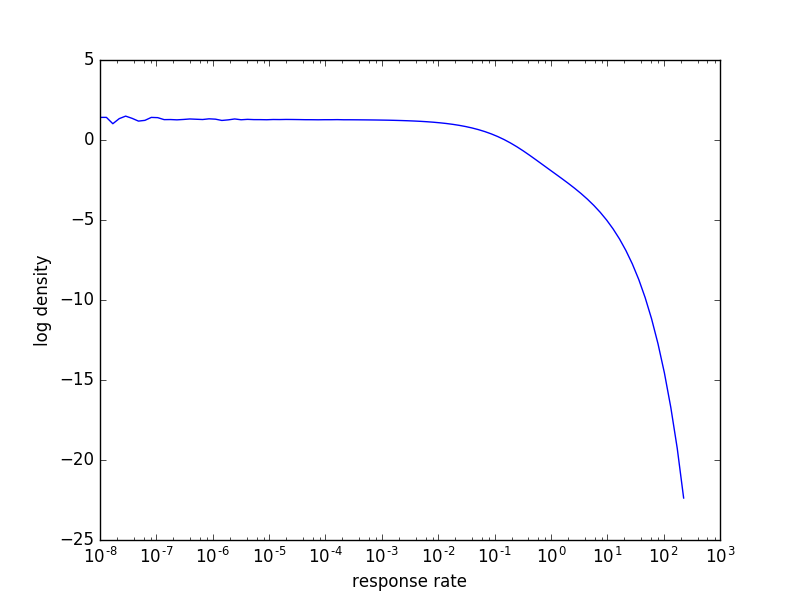
\includegraphics[width=0.47\textwidth, clip]{../pics/s2/margXLogDens_numeric_final}\\
\caption{Left column: Analytic solution. Right column: Numeric solution. Rows, top to bottom: Marginal (disrcretized) probability with logarithmically spaced values of $x$, marginal probability density, log of marginal probability density.}
\label{margs}
\end{figure}

\section{Posterior of contrast and orientation, given response}

Figure \ref{posts} shows the posterior probability of contrast and orientation, given a response rate. For low response rates the most likely stimulus is of non-preferred orientation, and has a higher contrast than the most likely stimulus with the preferred orientation. For higher response rates the posterior for the preferred stimulus orientation is highest.

\begin{figure}[h]
\centering
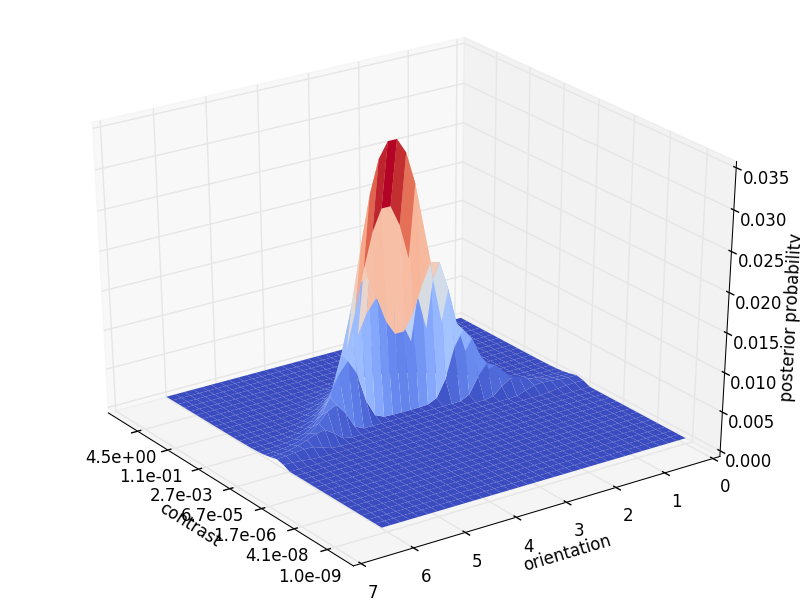
\includegraphics[width=0.49\textwidth, clip]{../pics/post_analytic_lowresp}
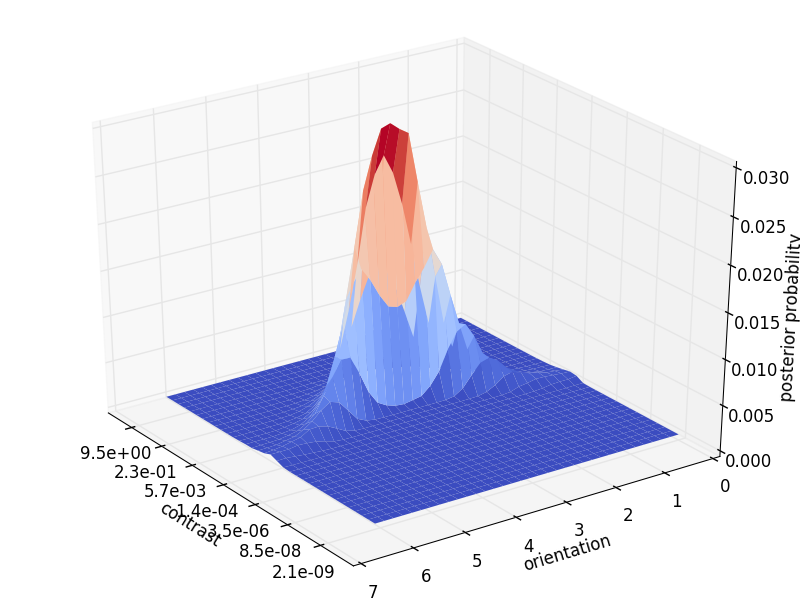
\includegraphics[width=0.49\textwidth, clip]{../pics/post_numeric_lowresp} \\
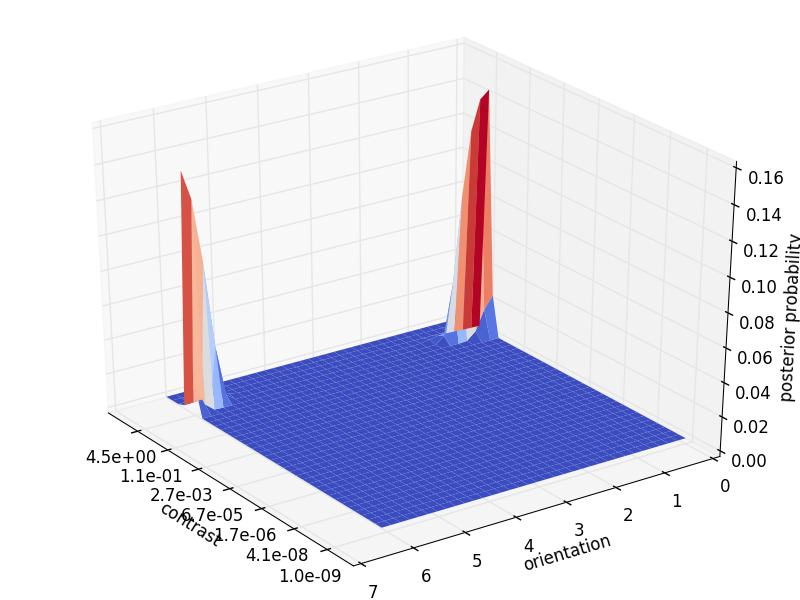
\includegraphics[width=0.49\textwidth, clip]{../pics/post_analytic_highresp}
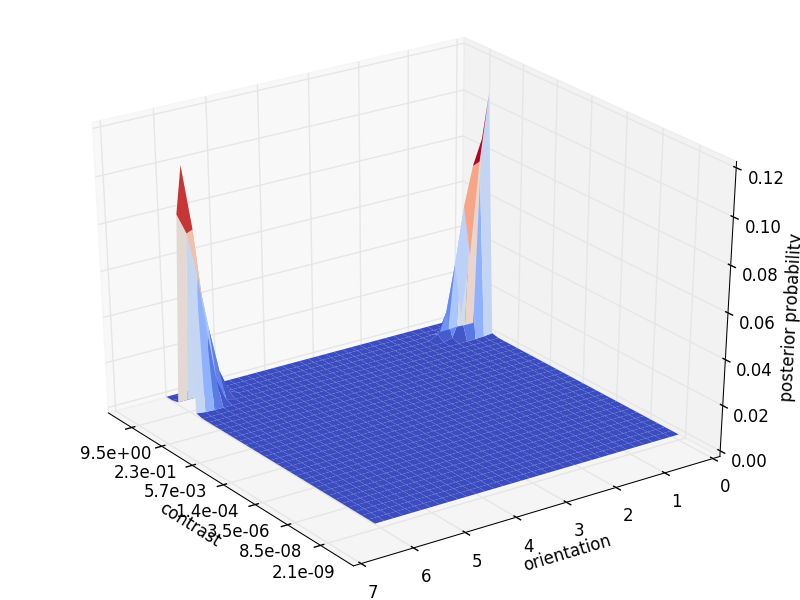
\includegraphics[width=0.49\textwidth, clip]{../pics/post_numeric_highresp}\\
\caption{Left column: Analytic solution. Right column: Numeric solution. Posterior distribution for $x_k=\num{6.7e-4}$ (top) and for $x_k=45.3$ (bottom). $c_0 = 1, \theta_k = 0$}
\label{posts}
\end{figure}

\section{Probability and latency of object detection}

I estimated the probability and latency of correctly detecting an object as a function of object duration and contrast. For a given sequence of stimuli and their response rates and a fixed window size I determined the most likely stimulus for every time step. The differences between true and detected contrast and orientation were transformed to be in the range $\left[0, 1\right]$. For the orientation I used the function $\operatorname{f}(\theta_s, \theta_d) = \frac{- \cos{(\theta_s - \theta_d)} + 1}{2}$ and for the contrast the function $\operatorname{f}(c_s, c_d) = \lvert \operatorname{cdf}(c_s, c_0) - \operatorname{cdf}(c_d, c_0) \rvert $ where subscripts $s$ and $d$ refer to the stimulus and detected values respectively and cdf is the cumulative density function for the distribution of stimulus contrast. If the result of these functions was smaller than a given threshold for both contrast and orientation at at least one point in time the corresponding stimulus was said to be correctly detected and the latency was set to the difference between stimulus onset and first time of correct detection.

Some example results are shown in Figure \ref{funs}. Overall trends appear to be as follows: Very low contrast and very high contrast objects are more difficult to detect than objects with average contrast. The latency is more or less independent of contrast, except for very high contrasts, where the latency is higher. Latency of detection is close to the worst possible value for short stimuli and otherwise independendent of stimulus duration. Probability of detection is high for all stimuli longer than the window size, with perhaps a small positive correlation between object duration and detection probability. For objects with a shorter duration than the window size the probability of detection rises rapidly with a longer duration. See also Figure \ref{sect}.

These results indicate that larger window sizes worsen detection performance. However this is only so because of the specific way of measuring the performance. Which stimulus is detected after a single correct inference is completely ignored. Because the variance of the inferred stimulus properties is larger for smaller window sizes, it is likelier to get the stimulus correct at least once, even if on average the error is larger.

\begin{figure}[h]
\centering
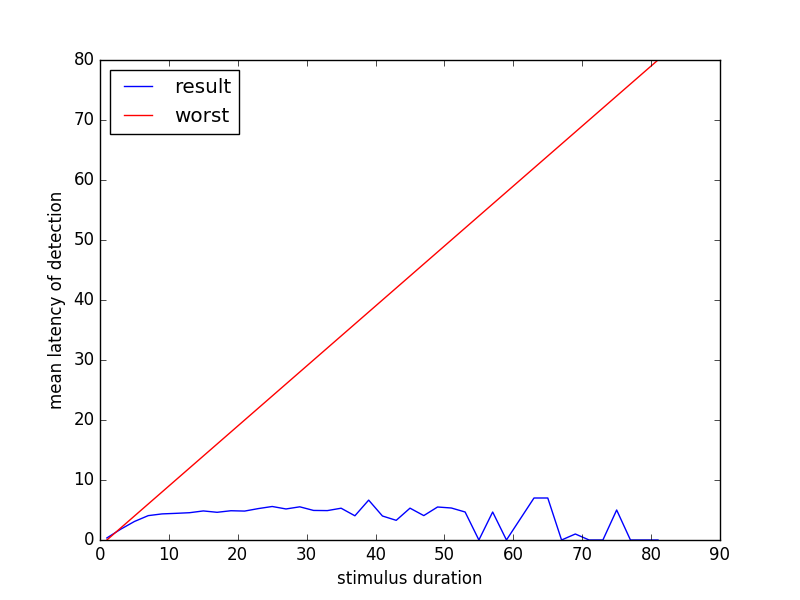
\includegraphics[width=0.47\textwidth, clip]{../pics/t4/latency_of_dur_4chans_1_8_8_01}
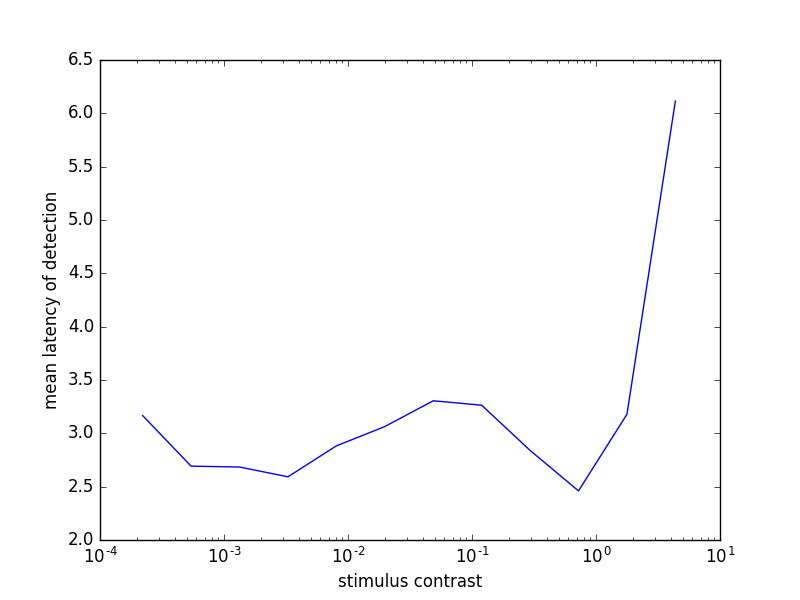
\includegraphics[width=0.47\textwidth, clip]{../pics/t4/latency_of_contr_4chans_1_8_8_01}\\
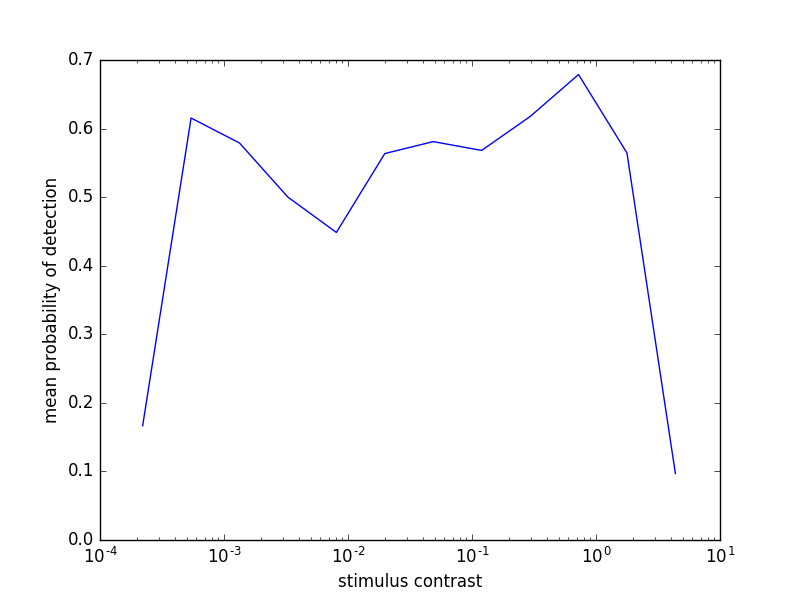
\includegraphics[width=0.47\textwidth, clip]{../pics/t4/prob_of_con_4chans_1_8_8_01}
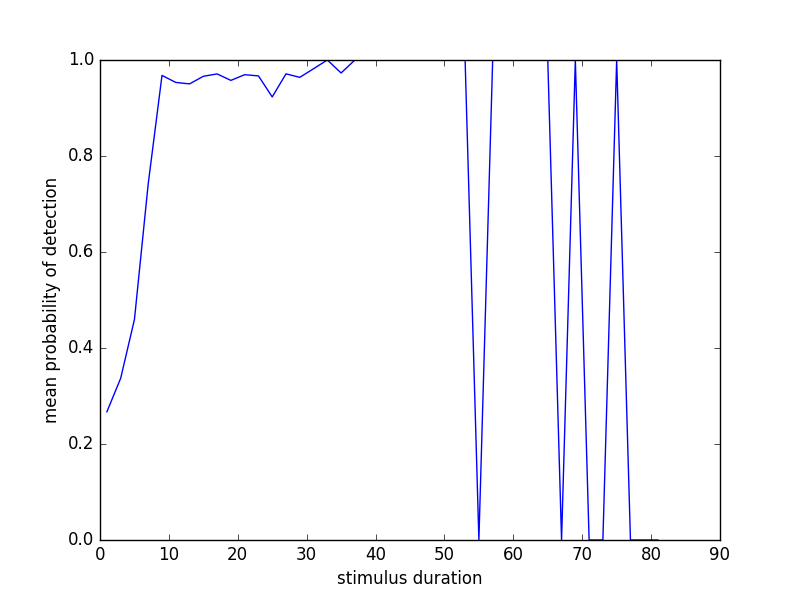
\includegraphics[width=0.47\textwidth, clip]{../pics/t4/prob_of_dur_4chans_1_8_8_01}\\
\caption{Probability and latency of stimulus detection as functions of stimulus duration and contrast. Chosen parameters: $c_0 = 1, \tau_0 = 8$, integration window size $=8$, detection threshold $=0.1$, number of channels $=4$. The red line in the top left plot indicates the maximum possible latency. Points on the line mean that the stimulus was either not detected at all, or detected at the last point in time before the next stimulus began. Actual results can be slightly above the line because the results for multiple durations are put together. The mean of zero values was set to zero, which explains the zero points in the bottom right plot.}
\label{funs}
\end{figure}

\begin{figure}
\centering
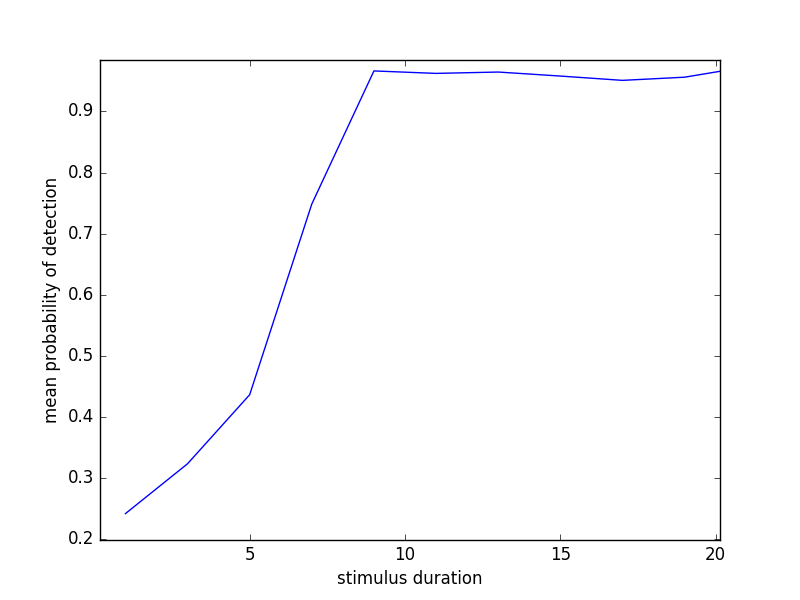
\includegraphics[width=0.66\textwidth, clip]{../pics/t4/prob_of_dur_1_8_8_01_section}
\caption{Chosen parameters: $c_0 = 1, \tau_0 = 8$, integration window size $=8$, detection threshold $=0.1$, number of channels $=12$. Illustration of the initial rapid rise of detection probability for stimuli shorter than the window size. }
\label{sect}
\end{figure}

\section{Standard deviaton of error}

std as performance index.
high std --> same stimulus is interpreted as being different
low std --> higher precision (can still be low accuracy)

\section{Optimal window size for parameters}

show some plots, high window size seems to be preferred too much? (longer stimuli are weighted stronger because they are longer, aggregate every separate stimulus into one? could do it once with prob/lat, once with std)

one optimizes for having long times of high accuracy, the other for getting many stimuli correct (enough), regardless of stimulus length

%\begin{align*}
%r_k =& c_s \exp{(2 \cos{\theta_k-\theta_s)}}\\
%\ln{\operatorname{p}(x_k, c_s, \theta_s)} =& 
%	\ln{\frac{\pi}{2} + 
%	\ln{x_k} - 
%	2 \ln{r_k} - 
%	\frac{\pi x_k^2}{4r_k^2} -
%	\ln{2\pi} - 
%	\frac{c_s}{c_0} - 
%	\ln{c_0}}\\	
%\operatorname{p} (x_k, c_s, \theta_s) =& 
%	\frac{x_k r_k}{4 c_0} \cdot 
%	\exp{\left( 
%		-\frac{\pi x_k^2}{4r_k^2} - 
%		\frac{c_s}{c_0} - 2 
%		\right)}\\	
%0 = \frac{\partial \operatorname{p} (x_k, c_s, \theta_s)}{\partial x_k} =& 
%	\frac{r_k}{4c_0} 
%	\exp{\left( 
%		-x_k^2 
%		\frac{\pi}{4r_k^2} - 
%		\frac{c_s}{c_0} - 2 
%		\right)} + 
%	\frac{x_k r_k}{4c_0}
%	\frac{-2\pi x_k}{4r_k^2} 
%	\exp{\left( 
%		-x_k^2 
%		\frac{\pi}{4r_k^2} 
%		\right) }\\	
%=& \underbrace{
%		\exp{\left( 
%			-x_k^2 
%			\frac{\pi}{4r_k^2}  
%			\right)}
%		\frac{r_k}{4c_0}}_{\neq 0} \cdot 
%	\left( 1 - 2\pi x_k^2 \right)\\
%x_k^2 =& \frac{1}{2\pi}\\
%x_k =& \sqrt{\frac{1}{2\pi}}\\ \\
%\operatorname{p}(\sqrt{1/2\pi}, c_s, \theta_s) =& 
%	\frac{c_s 
%		\exp{\left( 
%			2 \cos{\theta_k - \theta_s}
%			\right)}}
%		{4c_0\sqrt{2\pi}} \cdot
%	 \exp{\left(
%	 	-\frac{1}{8c_s}
%	 	\exp{\left(
%	 		-2\cos{\theta_k - \theta_s}
%	 		\right)}-
%	 	\frac{c_s}{c_0}-2
%	 	\right)} \\	 	
%0 = \frac{\partial \operatorname{p}(\sqrt{1/2\pi}, c_s, \theta_s)}{\partial \theta_s} =& \exp{\left(
%		-\frac{1}{8c_s}
%		\exp{\left(
%			-2\cos{\theta_k - \theta_s}
%			\right)} -
%		\frac{c_s}{c_0}-2
%		\right)} \cdot \\
%	&\frac{c_s 
%		\exp{\left(
%			2 \cos{\theta_k - \theta_s}
%			\right)}}
%		{4c_0\sqrt{2\pi}} 
%	\frac{2\sin{\theta_k-\theta_s}}{8c_s\exp{\left(
%		2\cos{\theta_k - \theta_s}
%		\right)}} \\
%+& \exp{\left(
%		-\frac{1}{8c_s}
%		\exp{\left(
%			-2\cos{\theta_k - \theta_s}
%			\right)} -
%		\frac{c_s}{c_0}-2
%		\right)} \cdot \\
%	 &\exp{\left(
%	 	2\cos{\theta_k - \theta_s}
%	 	\right)} 
%	 \frac{2c_s\sin{\theta_k-\theta_s}}{4c_0\sqrt{2\pi}} \\
%=& \underbrace{\exp{\left(
%		-\frac{1}{8c_s}
%		\exp{\left(
%			-2\cos{\theta_k - \theta_s}
%			\right)} -
%		\frac{c_s}{c_0}-2
%		\right)}
%	\exp{(2\cos{\theta_k-\theta_s})}
%	\frac{2c_s}{4c_0\sqrt{2\pi}}}_{\neq 0} \cdot \\
%	&\sin{(\theta_k-\theta_s)}
%	\underbrace{\left(
%		\frac{1}{8c_s} \exp{(-2\cos{(\theta_k-\theta_s)})}
%		+1
%		\right)}_{\neq 0}\\
%0 =& \sin{\theta_k - \theta_s} \\
%\theta_s =& \theta_k \\ \\
%\operatorname{p}(\sqrt{1/2\pi}, c_s, \theta_k) =& \frac{c_s e^2}{4c_0 \sqrt{2\pi}}
%	\exp{\left(
%		-\frac{1}{8c_se^2} - 
%		\frac{c_s}{c_0} - 2
%		\right)} \\
%0 = \frac{\partial \operatorname{p}(\sqrt{1/2\pi}, c_s, \theta_k)}{\partial c_s} =& 
%	\frac{c_s e^2}{4c_0 \sqrt{2\pi}}
%	\exp{\left(
%		-\frac{1}{8c_se^2} - 
%		\frac{c_s}{c_0} - 2
%		\right)}
%	\left(
%		-\frac{1}{c_0}
%		+ \frac{1}{8c_s^2e^2}
%		\right)	\\
%	+& \exp{\left(
%		-\frac{1}{8c_se^2} - 
%		\frac{c_s}{c_0} - 2
%		\right)}
%	\frac{e^2}{4c_0\sqrt{2\pi}} \\
%=& \underbrace{\left(
%	\exp{\left(
%		-\frac{1}{8c_se^2} - 
%		\frac{c_s}{c_0} - 2
%		\right)}
%	\frac{e^2}{4c_s\sqrt{2\pi}}
%	\right)}_{\neq 0} \cdot
%	\left(
%		\frac{1}{8c_se^2} - \frac{c_s}{c_0} + 1
%		\right)\\
%0 =& c_s^2 - c_sc_0 - \frac{c_0}{8e^2} \\
%c_s =& \frac{c_0}{2} +
%	\sqrt{
%		\frac{c_0^2}{4}+
%		\frac{c_0}{8e^2}}
%\end{align*}


\end{document}